\documentclass{beamer}
%\documentclass{powerdot}
%\documentclass{slides}[14pt]
%\pagestyle{empty}
%\normalsize
\usepackage{amsmath}
\usepackage{amssymb}
\usepackage{amscd}
% \usepackage{moreverb}
\usepackage{graphicx}
% \usepackage[all]{xy}
% \usepackage{beamerthemesplit}
\usepackage{moreverb}
\usepackage[all]{xy}

\input macros			   %% loan from John Gibson's snowbird 07 talk
% \input ../../inputs/defsThesis     %% all Vaggelis edits: \renewcommand, etc

% Setup appearance:

% \usetheme{Darmstadt}
\usefonttheme[onlylarge]{structurebold}
\setbeamerfont*{frametitle}{size=\normalsize,series=\bfseries}
\setbeamertemplate{navigation symbols}{}


% Standard packages

\usepackage[english]{babel}
\usepackage[latin1]{inputenc}
\usepackage{times}
\usepackage[T1]{fontenc}


% % Setup TikZ
% 
% \usepackage{tikz}
% \usetikzlibrary{arrows}
% \tikzstyle{block}=[draw opacity=0.7,line width=1.4cm]

\title{State-space geometry of a continuous symmetry reduced Kuramoto-Sivashinsky flow.}
\author{Evangelos Siminos}
\author[Siminos, Cvitanovi\'c, Davidchack]
{
  \textcolor{green!50!black}{Evangelos~Siminos}\inst{1} \and
  {Predrag~Cvitanovi\'c}\inst{1} \and
  {Ruslan~L.~Davidchack}\inst{2}
}
\institute
{
  \inst{1}%
  Georgia Institute of Technology
  \and
  \vskip-2mm
  \inst{2}%
  University of Leicester, United Kingdom
}
\date{May 19, 2009}

\begin{document}

\begin{frame}
  \titlepage
\end{frame}


\section[\KSe]{\KS, $L=22$, phase space }

\subsection{\KSe}

\begin{frame}{Abstract}

\small{
A dynamical description of spatially extended systems can be achieved by the study of the geometry of state-space in terms of compact, flow invariant objects. In systems with continuous symmetries such a description is obscured by the traveling nature of the solutions. We propose a scheme to implement symmetry reduction in high-dimensional truncations of partial differential equations and demonstrate its effectiveness in the context of Kuramoto-Sivashinsky equation, one of the simplest spatially extended systems with non-trivial dynamics. The procedure simplifies phase space visualization and provides new insight into the role that the unstable manifolds of equilibria and traveling waves play in organizing the flow. This in turn elucidates the mechanism that creates unstable modulated traveling waves (periodic orbits in reduced space) that provide a skeleton of the dynamics. Finally, the compact description of dynamics thus achieved sets the stage for reduction of the dynamics to mappings between a set of Poincar\'e sections.
}

\end{frame}


\begin{frame}{\KSe}
\[
  u_t = F(u) = -{\textstyle\frac{1}{2}}(u^2)_x-u_{xx}-u_{xxxx}
    \,,\qquad   x \in [-L/2,L/2]
    \,,
\]
Appears in study of many extended systems including
\begin{itemize}
 \item reaction-diffusion systems
 \item combustion problems (flame fronts)
 \item thin falling films
 \item drift waves in plasmas
 \item and more\ldots
\end{itemize}

\end{frame}


\begin{frame}{Symmetries of \KSe}

Impose periodic boundary conditions:
\[
 u(x,t) = u(x+L,t)
\]

Symmetry group $\On{2}$:
\begin{itemize}
%  \item Galilean invariance: if $u(x,t)$ is a solution, then $u(x-ct,t)-c$, with $c$ an arbitrary constant
% 	speed, is also a solution.
% 	\begin{itemize}
% 		\item The mean $u_0=\int_{-L/2}^{L/2} u dx$ is a constant of the motion. \\
% 		\item Setting $u_0=0$ corresponds to choosing $c=0$ therefore eliminating Galilean invariance.
% 	\end{itemize}
 \item Translations: $\Shift_{\shift/L}\, u(x,t) = u(x+\shift,t)\,,\qquad \shift\in\left[-L/2,L/2\right]\,,$
 \item Reflections:  $\Refl \, u(x) = -u(-x)\,.$
\end{itemize}

Due to translational symmetry: traveling wave solutions.

\begin{block}{Question} State-space geometry of a Kuramoto-Sivashinsky flow in terms of relative periodic orbits
What are the invariant objects that organize phase space in a spatially extended system 
with translational symmetry and \textcolor{green}{how do they fit together to form a
skeleton of the dynamics?}
\end{block}

% \begin{block}{Subspace of antisymmetric functions} 
% Pointwise invariant under $\Refl$: $\Refl u(x)=-u(-x)=u(x)$.\\
% (Christiansen et. al, Lan and Cvitanovi\'c) 
% \end{block}

\end{frame}



% \begin{frame}{Bifurcations}
% \begin{center}
%   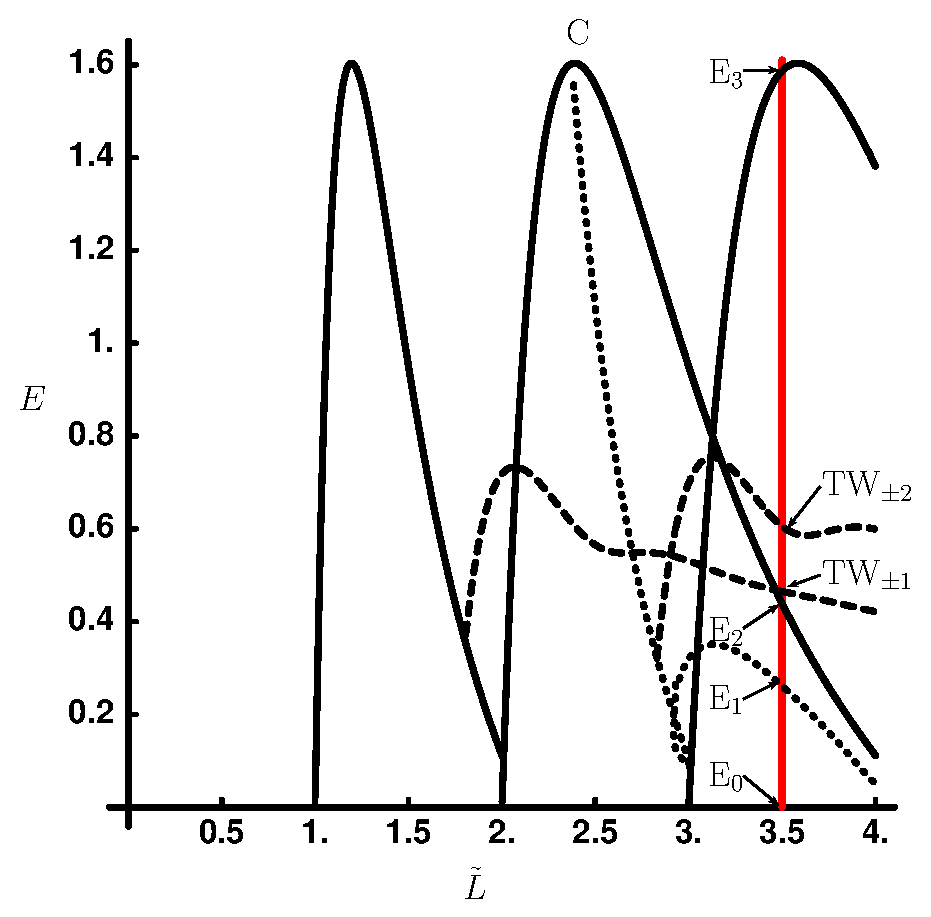
\includegraphics[width=0.5\textwidth]{../../figs/ksBifDiag}
% \end{center}
% \end{frame}

\begin{frame}{L=22}
\begin{center}
  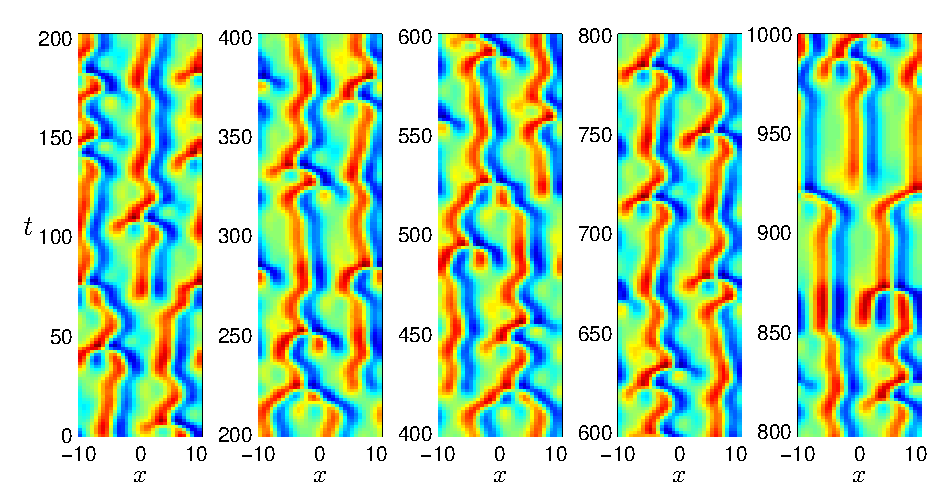
\includegraphics[width=0.9\textwidth]{../../figs/ks_L22_long_orbit}
\end{center}

\begin{block}{} 
 \begin{itemize}
  \item Lyapunov exponents: \\
	$(\lambda_i) = (0.048,$ 0, 0, $-0.003$, $-0.189$, $-0.256$, $-0.290$, $\cdots)$
  \item Non trivial but tractable.	
 \end{itemize}

\end{block}
 
\end{frame}

\begin{frame}{Fourier space}
Use
\[
  u(x,t)=\sum_{k=-\infty}^{+\infty} a_k (t) e^{ i q_k x }
\]
where
\[
 q_k = 2\pi\,k/L.
\]
Get
\[
 \dot{a}_k
     = ( q_k^2 - q_k^4 )\, a_k
    - i \frac{q_k}{2} \sum_{m=-\infty}^{+\infty} a_m a_{k-m}\,,
\]
with $a_{k}=a^\ast_{-k}$ since $u(x,t)$ is real.

Truncate to finite order $N$. Here $N=64$.
\end{frame}

\begin{frame}{Symmetry in Fourier space}

Symmetry acts as
\[
  \Shift_{\shift/L}\, a_k = e^{i q_k\, \shift} \, a_k \,,
  \label{eq:shiftF}
\]
\[
   \Refl \, a_k = -a_k^\ast
\]
where $q_k = 2\pi\,k/L$.

\end{frame}


\begin{frame}{Equilibria}
\begin{tabular}{ccc} ~~~\EQV{1} & ~~~\EQV{2} & ~~~\EQV{3} \vspace{12pt}\\
    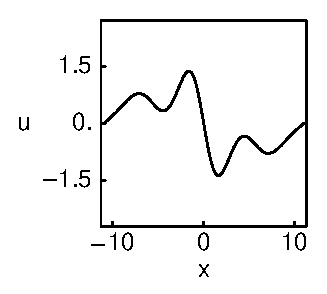
\includegraphics[width=0.25\textwidth]{../../figs/1wKS22equil}&
    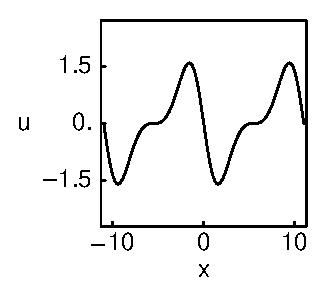
\includegraphics[width=0.25\textwidth]{../../figs/2wKS22equil}&
   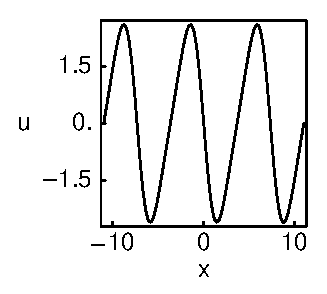
\includegraphics[width=0.25\textwidth]{../../figs/3wKS22equil}
\end{tabular}

\begin{itemize}
 \item All live in subspace $\bbU$ of antisymmetric functions, 
  pointwise invariant under $\Refl$: $\Refl u(x)=-u(-x)=u(x)$.
 \item $\EQV{2}$ invariant under $\Shift_{1/2}$.
 \item $\EQV{3}$ invariant under $\Shift_{1/3}$.
 \item For any $\EQV{i}$ we have a continuous family of equilibria under rotations $\Shift_{\shift/L}\,\EQV{i}$.
 \item The copies live in $\Shift_{\shift/L}\,\bbU$.
\end{itemize}

\end{frame}

\begin{frame}{Traveling Waves}
 \begin{columns}
 \column{0.5\textwidth}
%  \begin{tabular}{cc}
 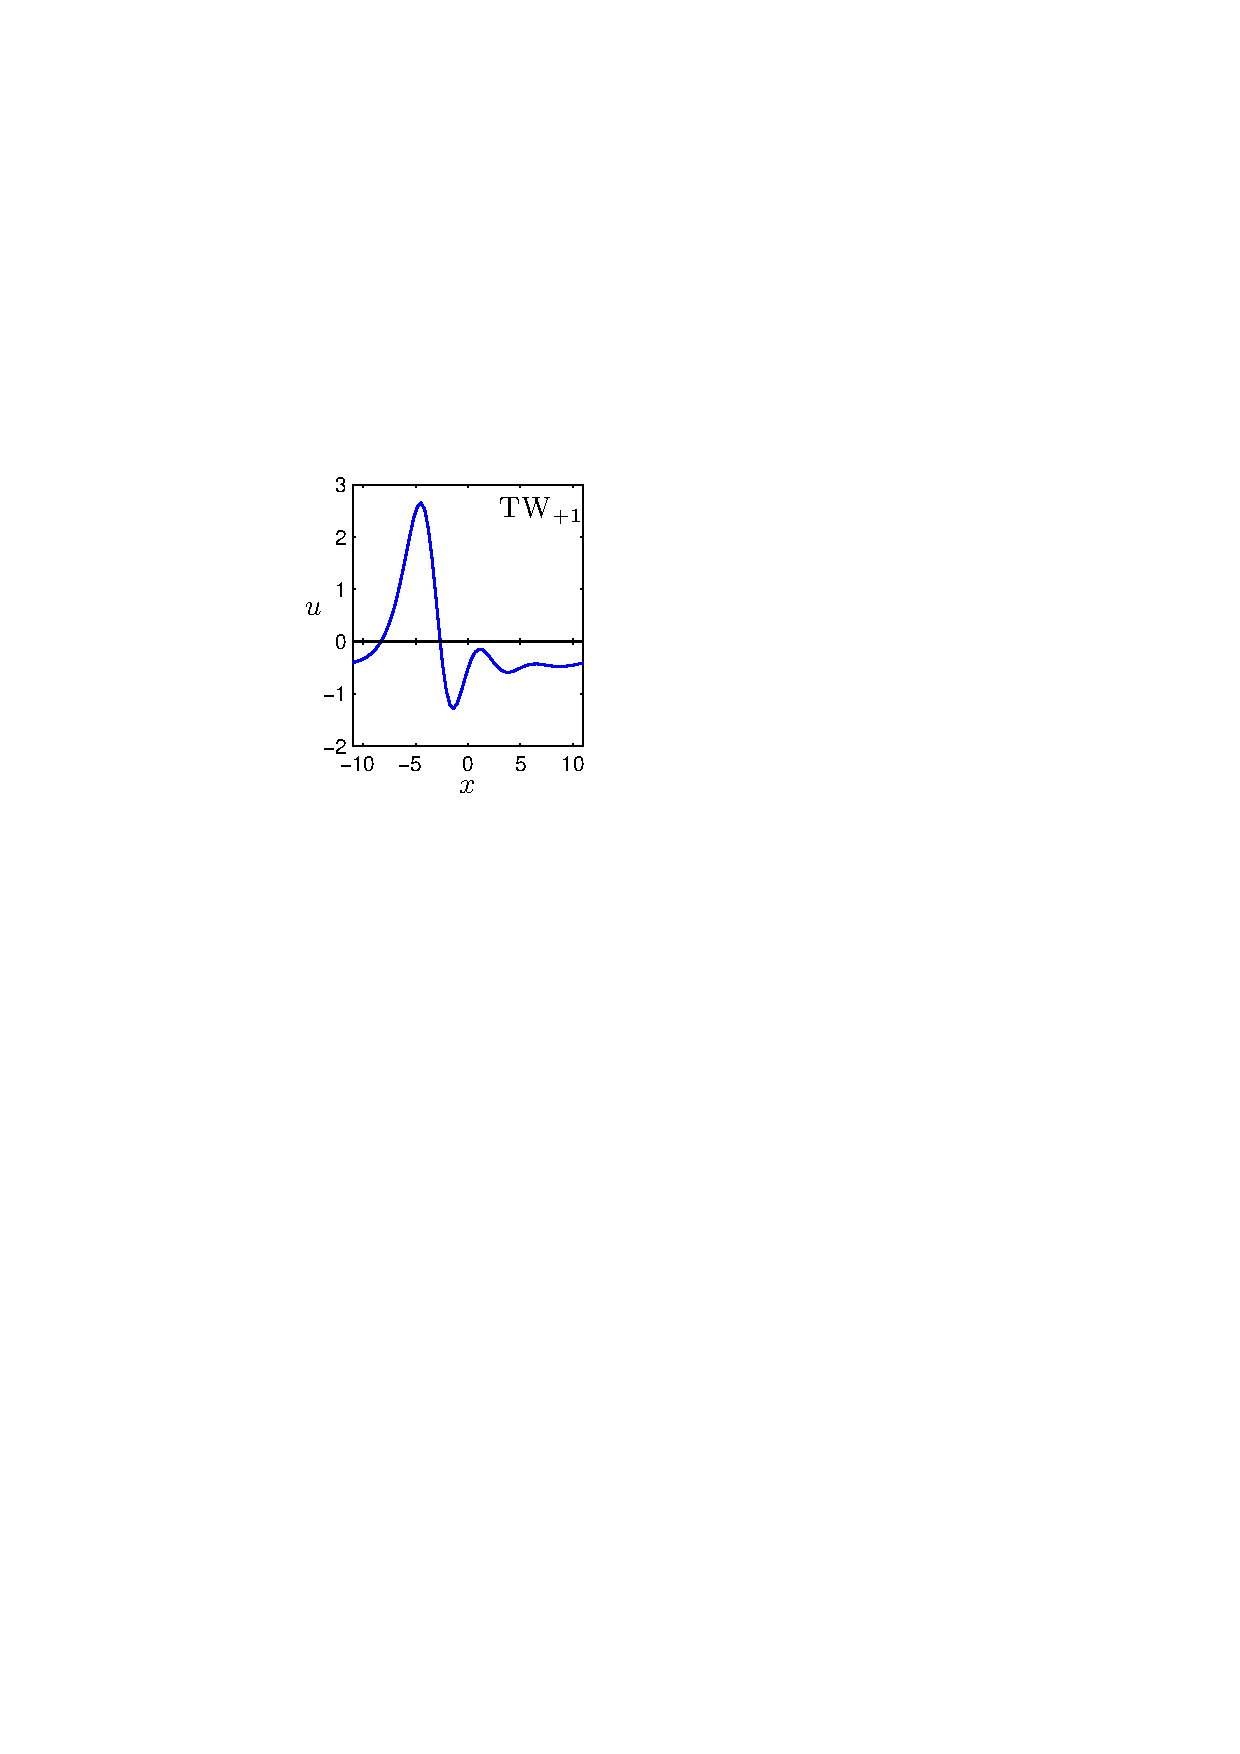
\includegraphics[width=0.6\textwidth]{../../figs/ks22_TW1_profile}\\
 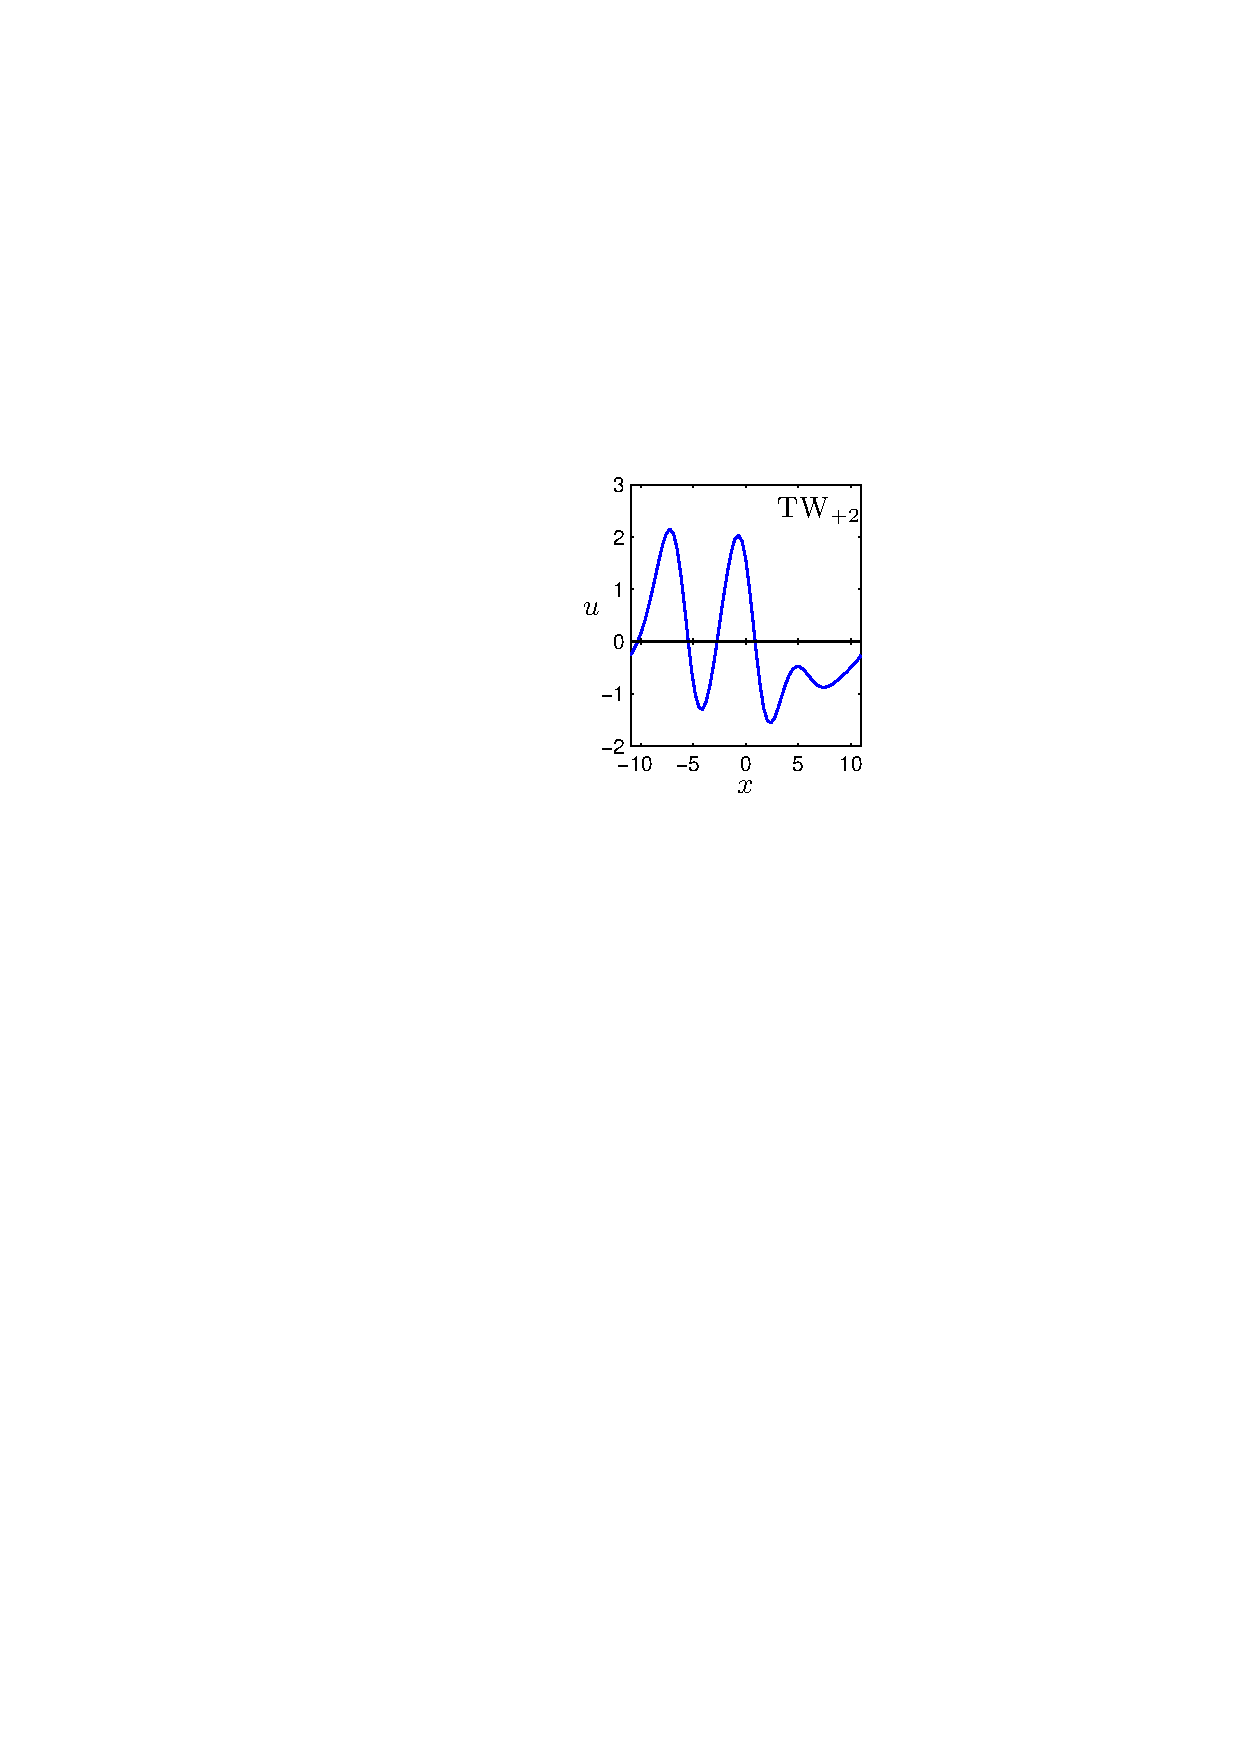
\includegraphics[width=0.6\textwidth]{../../figs/ks22_TW2_profile}%\\
%  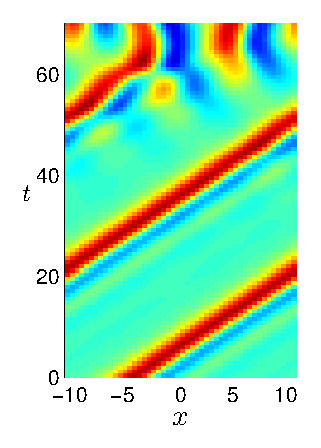
\includegraphics[width=0.5\textwidth]{../../figs/ks22_TW1_orbit_c}
%  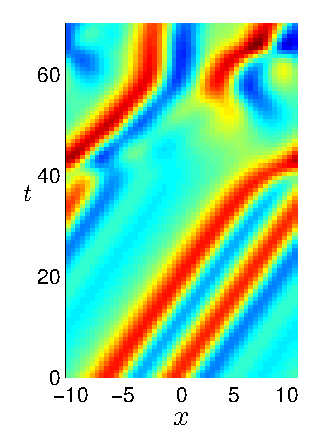
\includegraphics[width=0.5\textwidth]{../../figs/ks22_TW2_orbit_c}
%  \end{tabular}
 \column{0.5\textwidth}
 \begin{itemize}
 \item Invariant (as a set) under rotations: relative equilibria.
 \item Come in counter-traveling pairs related by reflections.
 \item They live in full space.
\end{itemize}

 \end{columns}
\end{frame}

% \begin{frame}{Unstable manifolds: \EQV{1}}
%  \begin{tabular}{cc}
%  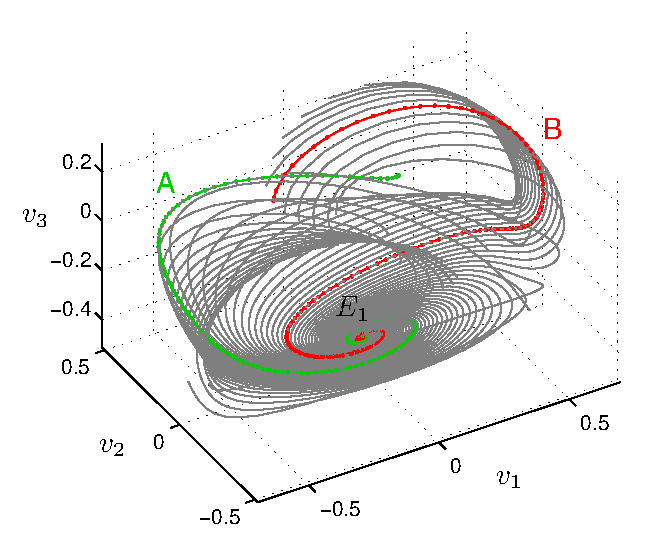
\includegraphics[width=0.3\textwidth]{../../figs/ks22_E1_plane1_manifold_c} &
%  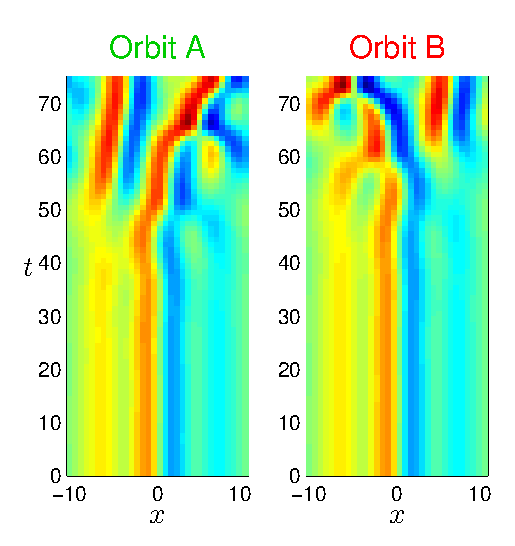
\includegraphics[width=0.2\textwidth]{../../figs/ks22_E1_plane1_orbits_c}\\
%  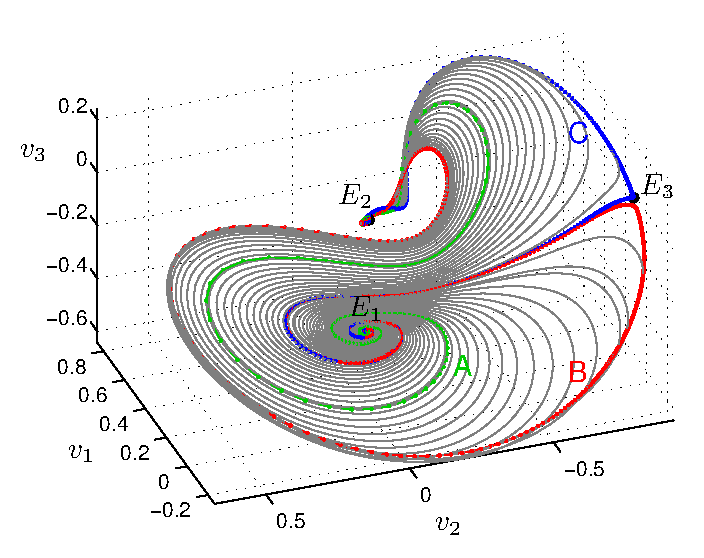
\includegraphics[width=0.3\textwidth]{../../figs/ks22_E1_plane2_manifold_c} &
%  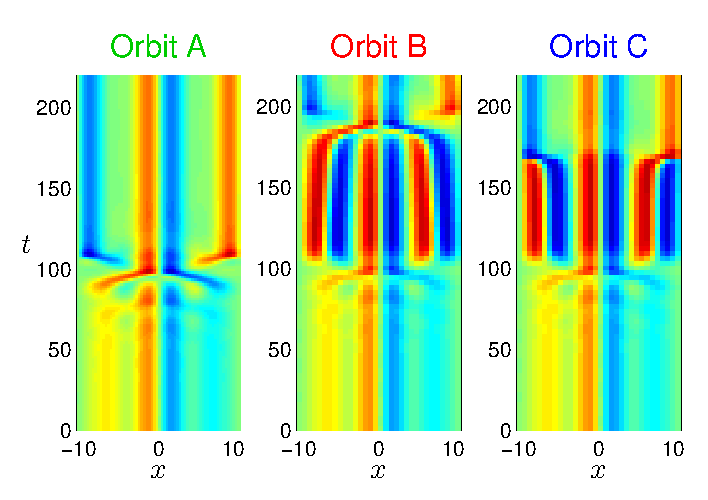
\includegraphics[width=0.32\textwidth]{../../figs/ks22_E1_plane2_orbits_c}
%  \end{tabular}
% \end{frame}


\begin{frame}{Unstable \rpo s}


\Rpo s (modulated traveling waves) satisfy:
\[
  \Shift_{\shift_p/L}u(x,\period{p}) =
  u(x+\shift_p,\period{p}) = u(x,0) = u_p(x)\,.
\]
\Po s satisfy:
\[
   \Refl u(x+\shift,\period{p}) =
  -u(-x-\shift,\period{p}) = u(x+\shift,0) = u_p(x)
\]

For \KSe\ bifurcation branches of \rpo s have been studied in detail by Brown and Kevrekidis (1996).

\end{frame}

\begin{frame}{Unstable \rpo s}

\scriptsize
 \begin{tabular}{ccccc} 
~~~$\period{p} = 16.3$, & ~~~$\period{p} = 33.5$,  & ~~~$\period{p} = 47.6$,  &
%                          ~~~$\period{p} = 71.7$,  & 
~~~$\period{p} = 10.3$ & ~~~$\period{p} = 33.4$\\
~~~$\shift_p = 2.86$ & ~~~$\shift_p = 4.04$ & ~~~$\shift_p = 5.68$ & 
% ~~~$\shift_p = 5.503$ & 
&\\
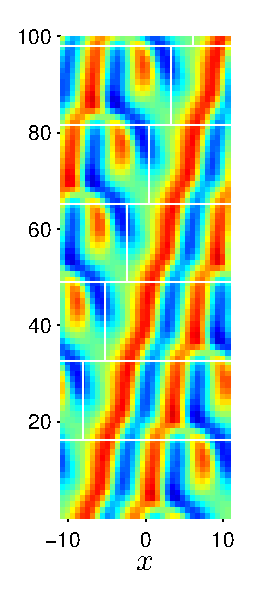
\includegraphics[width=0.15\textwidth]{../../figs/ks22rpo016.3-02.86.eps}\hspace{-3ex} &
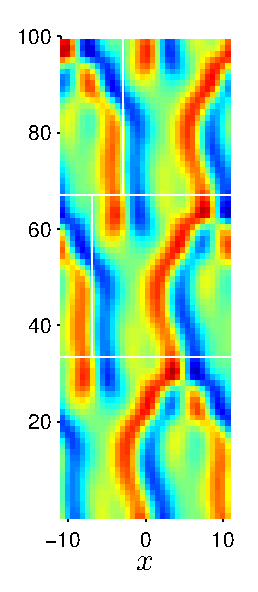
\includegraphics[width=0.15\textwidth]{../../figs/ks22rpo033.5-04.04.eps}\hspace{-3ex} &
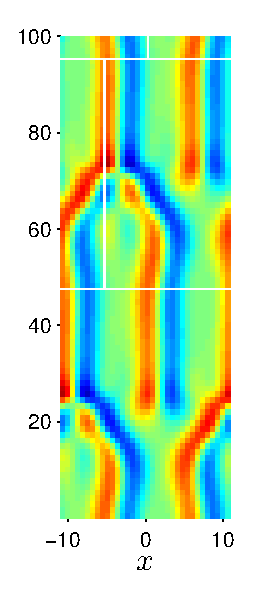
\includegraphics[width=0.15\textwidth]{../../figs/ks22rpo047.6-05.68.eps}\hspace{-3ex} &
% 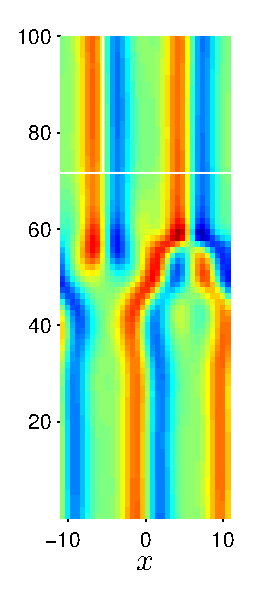
\includegraphics[width=0.15\textwidth]{../../figs/ks22rpo071.7-05.50.eps}\hspace{-3ex} &
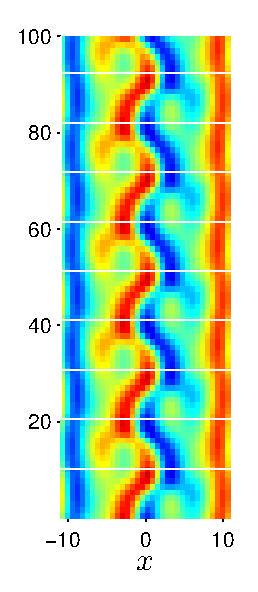
\includegraphics[width=0.15\textwidth]{../../figs/ks22rpo020.5-00.00.eps}\hspace{-3ex} &
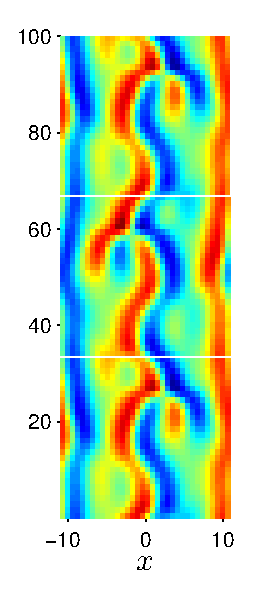
\includegraphics[width=0.15\textwidth]{../../figs/ks22rpo066.8-00.00.eps}\\
% $\period{p} = 32.8$, $\shift_p = 10.96$ & $\period{p} = 34.6$, $\shift_p = 9.60$ & $\period{p} = 59.9$, $\shift_p = 5.44$ &
% $\period{p} = 84.4$, $\shift_p = 5.513$ & $\period{p} = 32.4$ & $\period{p} = 35.2$\\
% 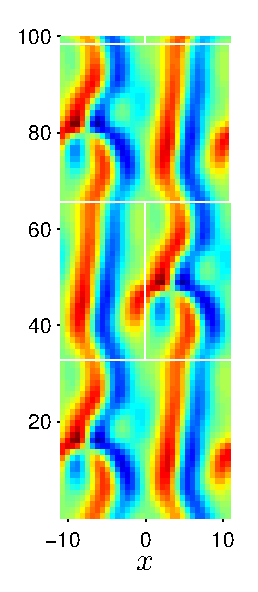
\includegraphics[width=0.15\textwidth]{../../figs/ks22rpo032.8-10.96.eps}\hspace{-3ex} &
% 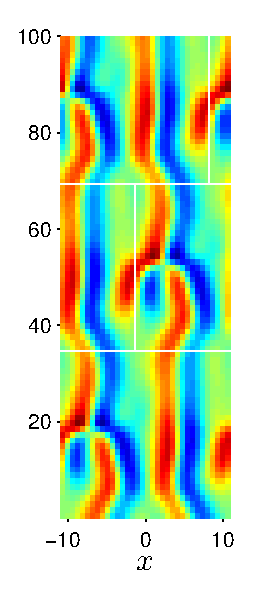
\includegraphics[width=0.15\textwidth]{../../figs/ks22rpo034.6-09.60.eps}\hspace{-3ex} &
% 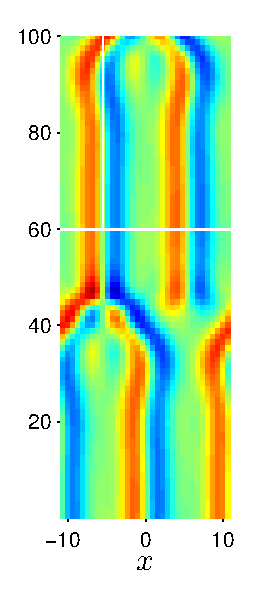
\includegraphics[width=0.15\textwidth]{../../figs/ks22rpo059.9-05.44.eps}\hspace{-3ex} &
% 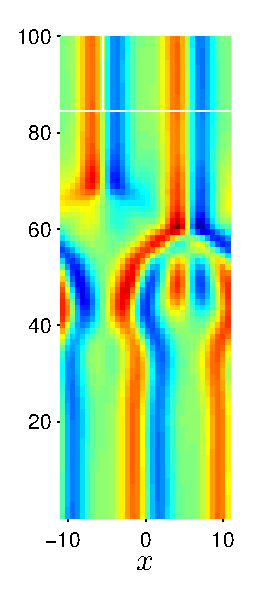
\includegraphics[width=0.15\textwidth]{../../figs/ks22rpo084.4-05.51.eps}\hspace{-3ex} &
% 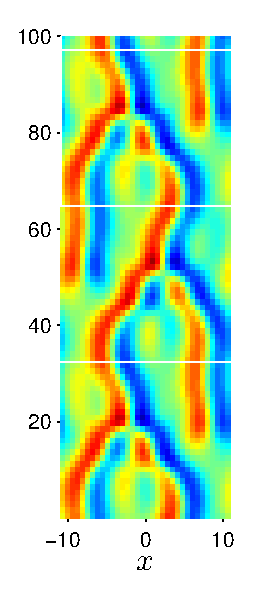
\includegraphics[width=0.15\textwidth]{../../figs/ks22rpo064.7-00.00.eps}\hspace{-3ex} &
% 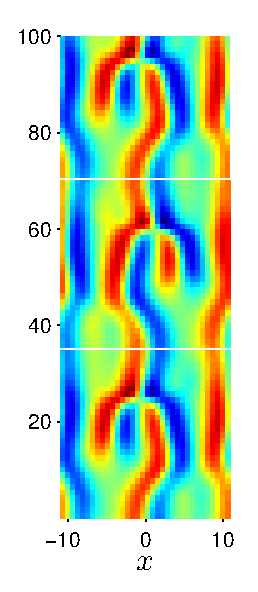
\includegraphics[width=0.15\textwidth]{../../figs/ks22rpo070.3-00.00.eps}

\end{tabular}

\begin{itemize}
 \item Located 30,000 unstable periodic and \rpo s through multiple shooting. See 
	Cvitanovi{\'c}, Davidchack and Siminos (2009), for details.
 \item How are they organized?
\end{itemize}

 
\end{frame}

\begin{frame}{Linear stability of {\eqva} and \reqva.}
\begin{center} %\footnotesize
\begin{tabular}{cccc}
\EQV{1}& $\Re{\lambda}$ & $\Im{\lambda}$ & Symmetry \\\hline
   & $\ \ 0.1308$& $0.3341$ & -  \\
   & $\ \ 0.0824$& $0.3402$ & $\bbU$  \\
\EQV{2}&  &  & \\\hline
   & $\ \ 0.1390$& $0.2384$ & $\bbU$         \\
\EQV{3}&  &   \\\hline
     &$\ \ 0.0933$&          & $\bbU$     \\
     &$\ \ 0.0933$&          & -           \\
$\REQV{\pm}{1}$&  &   \\\hline
   & $\ \ 0.1156$ & $0.8173$ & -  \\
   & $\ \ 0.0337$ & $0.4189$ & -  \\
$\REQV{\pm}{2}$&  &   \\\hline
     & $\ \ 0.3370$ &          & -  \\
\end{tabular}
\end{center}
%   \column{0.5\textwidth}
%   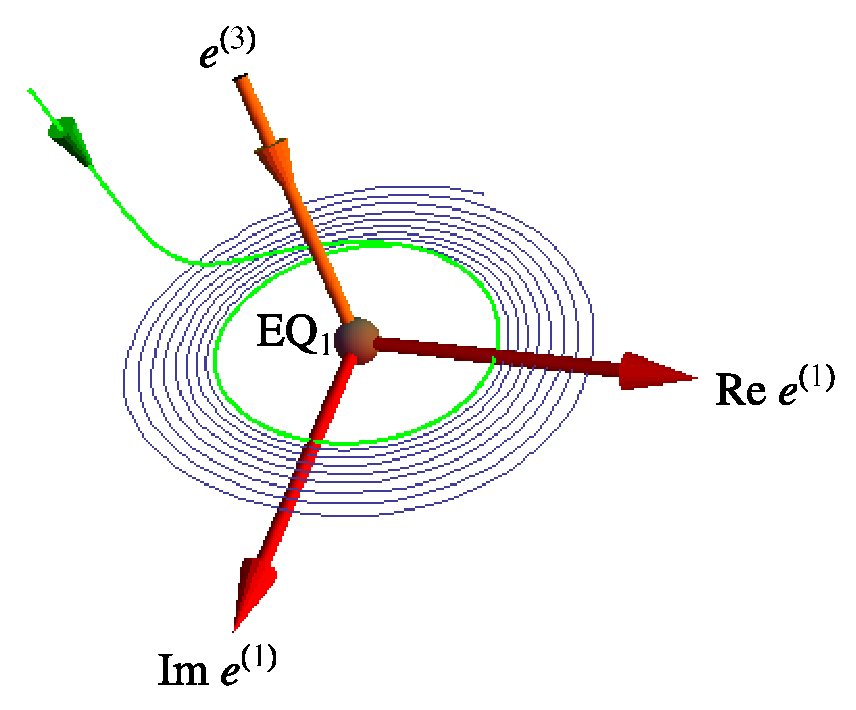
\includegraphics[width=\textwidth, crop=true]{../../figs/lorenzPolarManifDetail1.eps}
\end{frame}


\begin{frame}{Unstable manifolds: \EQV{2}}
 \begin{columns}
  \column{0.5\textwidth}
	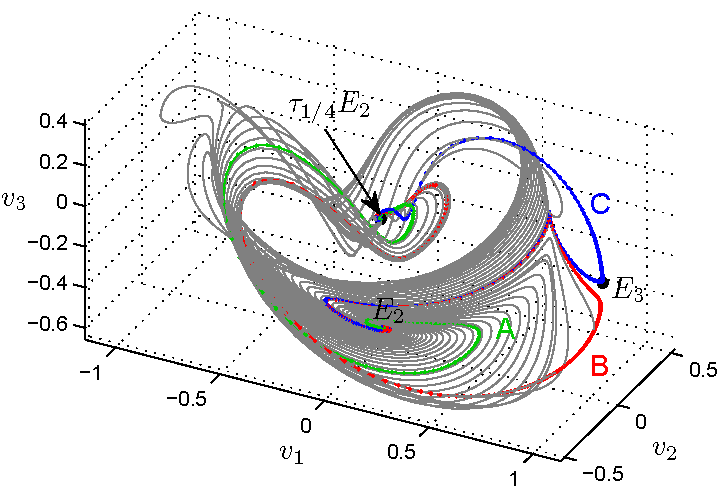
\includegraphics[width=\textwidth,height=0.6\textheight]{../../figs/ks22_E2_manifold_c}\\
	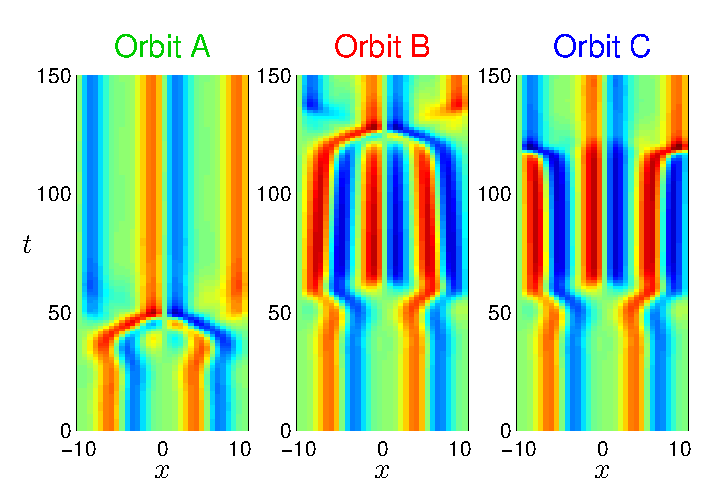
\includegraphics[width=0.8\textwidth,height=0.3\textheight]{../../figs/ks22_E2_orbits_c}		
 \column{0.5\textwidth}
 \begin{itemize}
  \item Heteroclinic connections in \KSe\ are robust (Kevrekidis et. al. (1990), Armbruster et. al. (1989)).
  \item Unstable manifolds stay in $\bbU$ (but with rotated copies in $\Shift_{\shift/L}\bbU$.
  \item For visualization we project to the leading stability eigenvectors (inspired by Gibson et. al. 2008).
 \end{itemize}
 \end{columns}
	
\end{frame}

% \begin{frame}{Unstable manifolds: \EQV{3}}
%  \begin{tabular}{cc}
%  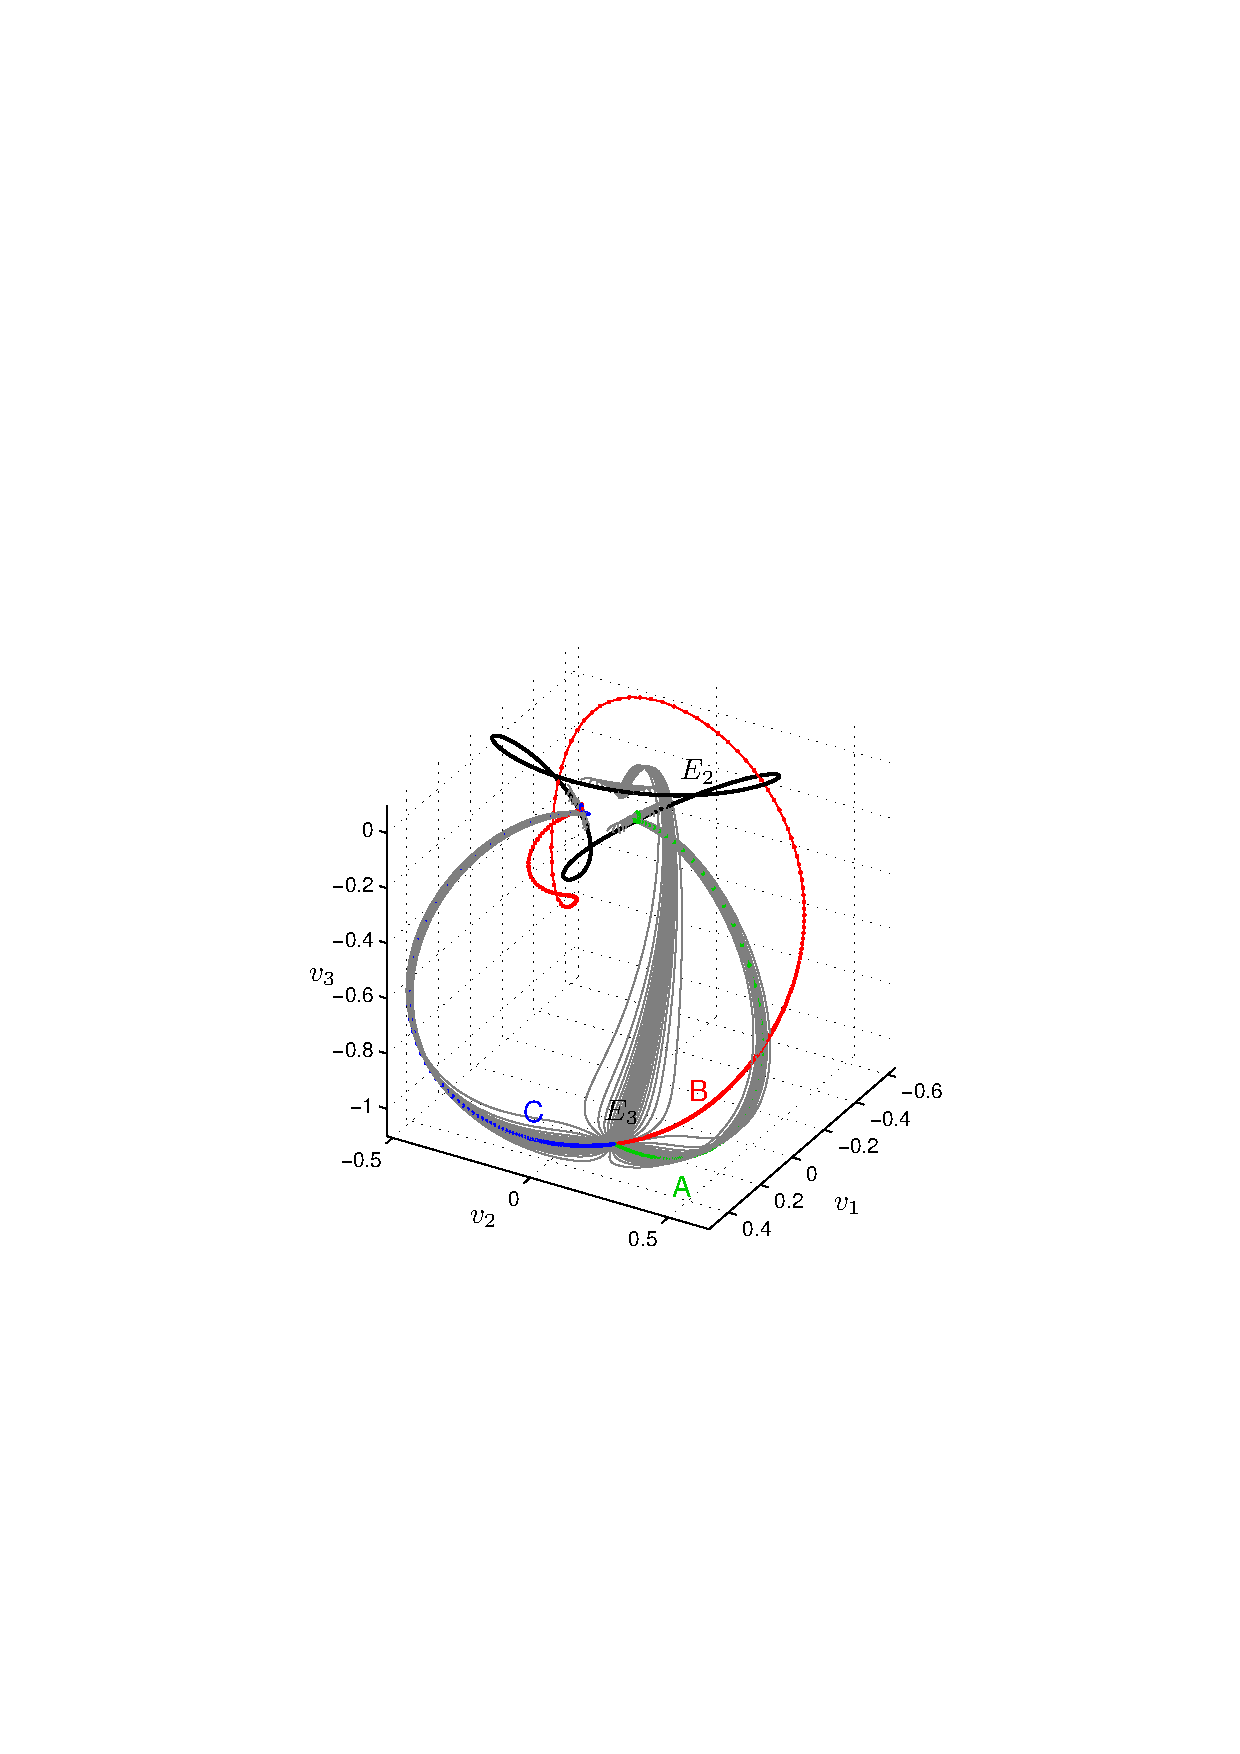
\includegraphics[width=0.45\textwidth]{../../figs/ks22_E3_manifold}
%  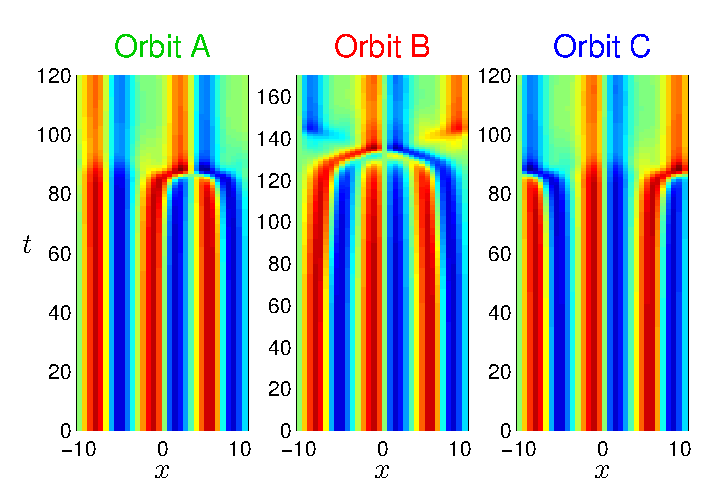
\includegraphics[width=0.5\textwidth]{../../figs/ks22_E3_orbits_c}	
%  \end{tabular}
% \end{frame}

\begin{frame}{Dynamics in antisymmetric subspace}
 \begin{centering}
         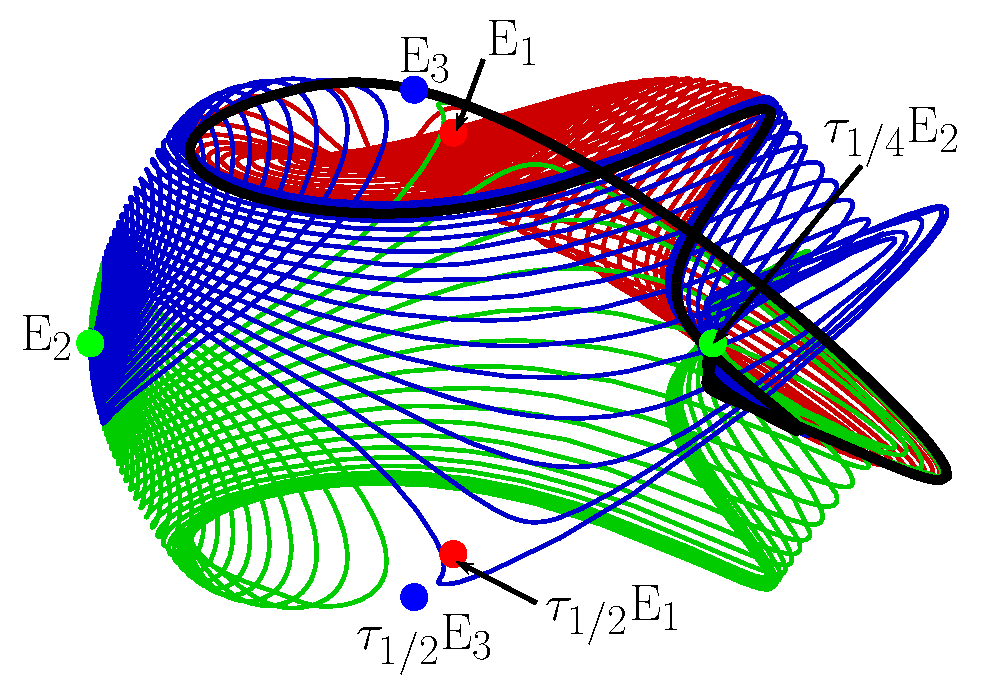
\includegraphics[width=0.6\textwidth]{../../figs/KS22hetero} \\
	Projection from $128$ dimensions onto the plane given by the vectors 
	$\EQV{2}-\Shift_{1/4}\EQV{2}$ and $\EQV{3}-\Shift_{1/2}\EQV{3}$ (inspired by Gibson et. al. 2008).
 \end{centering}
\end{frame}

\section[Symmetry reduction]{Symmetry reduction}

\subsection{Symmetry reduction}

\begin{frame}{Symmetry reduction}
\begin{itemize}
 \item All points related by a symmetry operation are mapped to the same point.
 \item Relative equilibria become equilibria and relative periodic orbits become periodic orbits in reduced space.
 \item Families of solutions are mapped to a single solution.
\end{itemize}
\end{frame}


% \begin{frame}{Reduction methods}


% \end{frame}

\begin{frame}{Reduction methods}

\begin{itemize}
	\item Integrate in directions transverse to the direction of group action at a point $x_0$. \textcolor{red}{Local.}\\
	(Rowley and Marsden (2000)).
 \item<alert@1> Rewrite the equations in variables invariant under the symmetry transformation
%  \only<2->{\item<alert@1> Rewrite the equations in variables that do not change (are invariant) under the symmetry transformation.}
 \item or compute solutions in original space and map them to invariant variables.
 \item How do we find those variables?
	\begin{itemize}
	\item<alert@1> Invariant polynomials (Hilbert basis): computationaly prohibitive for high-dimensional flows.
	\item<alert@1> Moving frame method by Cartan, reformulated by Fels and Olver (1999): singularities.
	\end{itemize}
\end{itemize}

\end{frame}

% \begin{frame}{Moving frame method}
%  \begin{block}{Idea}
%   	\begin{itemize}
%  		\item Introduce a \emph{cross-section}: A hypersurface that intersects all group
% 			orbits of a point exactly once.
% 		\item Then given a point $x$ find a map that tells you the transformation parameter(s)
% 			needed to bring $x$ to the cross-section. This is called a moving frame.
% 	\end{itemize}
%  \end{block}
% 
%  \begin{block}{For \CLe}
% 	\begin{description}
%  		\item{Cross-section} $x_1=0$, $x_2>0$.
% 		\item{Moving frame} $\theta=\tan^{-1}\frac{x_1}{x_2}$.
% 	\end{description}
%   	
%  \end{block}

 
% \end{frame}

% \begin{frame}{Moving frame method}
% 
% % \[
% % 	\left(\barr{cc} \overline{b}_k \\ \overline{c}_k\earr \right)=\left(\barr{cc}
% % 			    			\cos(k\theta) & -\sin(k\theta)\\
% % 						\sin(k\theta) & \cos(k\theta)\\
% % 			   			\earr\\	
% % 						\right) \left(\barr{cc} b_k \\ c_k\earr\right)\,,\ \ k=1,\ldots N\,.
% % \]
% % with $a_k=b_k+i c_k\,,\ b_k,c_k\in\Rls{}$.
% \end{frame}

\begin{frame}{Moving frame method}
  \begin{block}{}
	\begin{itemize}
	\item Write out group transformations explicitly:
	\[
	 \left(\barr{cc} \overline{b}_k \\ \overline{c}_k\earr \right)=\left(\barr{cc}
			    			\cos(k\theta) & -\sin(k\theta)\\
						\sin(k\theta) & \cos(k\theta)\\
			   			\earr	
						\right)\left(\barr{cc} b_k \\ c_k\earr\right)\,,\ \ k=1,\ldots N\,.
	\]
	\item Define a \emph{cross-section}:
	\[
 		K_1(a)=c_1=0\,,\qquad b_1>0\,
	\]
	\item Find the group element that brings a point back to the cross-section:
	\[
		\theta=-\tan^{-1}\frac{c_1}{b_1}\,,	
	\]
	\end{itemize}
  \end{block}
\end{frame}

\begin{frame}{Invariants}
  \begin{block}{}
\only<1>{
	\[
	\begin{array}{ll}
	u_1=r_1=\sqrt{b_1^2+c_1^2}&  \\ 
	u_3=\frac{b_2 \left(b_1^2-c_1^2\right)+2 b_1 c_1 c_2}{r_1^2}& \\
	u_4=\frac{-2
	b_1 b_2 c_1+\left(b_1^2-c_1^2\right) c_2}{r_1^2} & \\ 
	u_5=\frac{b_1 b_3 \left(b_1^2-3 c_1^2\right)-c_1 \left(-3
	b_1^2+c_1^2\right) c_3}{r_1^3}& \\ 

	u_6=\frac{-3 b_1^2 b_3 c_1+b_3 c_1^3+b_1^3 c_3-3 b_1 c_1^2 c_3}{r_1^3} & \\ 
	u_7=\frac{b_4
 	\left(b_1^4-6 b_1^2 c_1^2+c_1^4\right)+4 b_1 c_1 \left(b_1^2-c_1^2\right) c_4}{r_1^4}& \\ 
	u_8=\frac{4 b_1
 	b_4 c_1 \left(-b_1^2+c_1^2\right)+\left(b_1^4-6 b_1^2 c_1^2+c_1^4\right) c_4}{r_1^4}
% \\ u_9=\frac{b_1
% 	b_5 \left(b_1^4-10 b_1^2 c_1^2+5 c_1^4\right)+c_1 \left(5 b_1^4-10 b_1^2 c_1^2+c_1^4\right) c_5}{r_1^5}&u_{10}=\frac{-b_5
% 	c_1 \left(5 b_1^4-10 b_1^2 c_1^2+c_1^4\right)+b_1 \left(b_1^4-10 b_1^2 c_1^2+5 c_1^4\right) c_5}{r_1^5}\\ u_{11}=\frac{b_6
% 	\left(b_1^6-15 b_1^4 c_1^2+15 b_1^2 c_1^4-c_1^6\right)+2 b_1 c_1 \left(3 b_1^4-10 b_1^2 c_1^2+3 c_1^4\right) c_6}{r_1^6}&u_{12}=\frac{-2
% 	b_1 b_6 c_1 \left(3 b_1^4-10 b_1^2 c_1^2+3 c_1^4\right)+\left(b_1^6-15 b_1^4 c_1^2+15 b_1^2 c_1^4-c_1^6\right) c_6}{r_1^6}\\
	\end{array}
	\]
}
\only<2>{
	\[
	\begin{array}{ll}
	u_1=r_1=\sqrt{b_1^2+c_1^2}&  \\ 
	u_3=\frac{b_2 \left(b_1^2-c_1^2\right)+2 b_1 c_1 c_2}{\textcolor{green}{r}^2}& \\
	u_4=\textcolor{green}{\sqrt{b_2^2+c_2^2}}+\frac{-2
	b_1 b_2 c_1+\left(b_1^2-c_1^2\right) c_2}{\textcolor{green}{r}^2} & \\ 
	u_5=\textcolor{green}{\sqrt{b_3^2+c_3^2}}+\frac{b_1 b_3 \left(b_1^2-3 c_1^2\right)-c_1 \left(-3
	b_1^2+c_1^2\right) c_3}{\textcolor{green}{r}^3}& \\ 
	u_6=\frac{-3 b_1^2 b_3 c_1+b_3 c_1^3+b_1^3 c_3-3 b_1 c_1^2 c_3}{\textcolor{green}{r}^3} & \\ 
	u_7=\frac{b_4
 	\left(b_1^4-6 b_1^2 c_1^2+c_1^4\right)+4 b_1 c_1 \left(b_1^2-c_1^2\right) c_4}{\textcolor{green}{r}^4}& \\ 
	u_8=\textcolor{green}{\sqrt{b_4^2+c_4^2}}+\frac{4 b_1
 	b_4 c_1 \left(-b_1^2+c_1^2\right)+\left(b_1^4-6 b_1^2 c_1^2+c_1^4\right) c_4}{\textcolor{green}{r}^4}
% \\ u_9=\frac{b_1
% 	b_5 \left(b_1^4-10 b_1^2 c_1^2+5 c_1^4\right)+c_1 \left(5 b_1^4-10 b_1^2 c_1^2+c_1^4\right) c_5}{r_1^5}&u_{10}=\frac{-b_5
% 	c_1 \left(5 b_1^4-10 b_1^2 c_1^2+c_1^4\right)+b_1 \left(b_1^4-10 b_1^2 c_1^2+5 c_1^4\right) c_5}{r_1^5}\\ u_{11}=\frac{b_6
% 	\left(b_1^6-15 b_1^4 c_1^2+15 b_1^2 c_1^4-c_1^6\right)+2 b_1 c_1 \left(3 b_1^4-10 b_1^2 c_1^2+3 c_1^4\right) c_6}{r_1^6}&u_{12}=\frac{-2
% 	b_1 b_6 c_1 \left(3 b_1^4-10 b_1^2 c_1^2+3 c_1^4\right)+\left(b_1^6-15 b_1^4 c_1^2+15 b_1^2 c_1^4-c_1^6\right) c_6}{r_1^6}\\
	\end{array}
	\]
}
  \end{block}

\only<2>{\begin{block}{}
	\scriptsize
	\[
          r=\sqrt{\sum_{i=1}^N b_i^2+c_i^2}
	\]
         \end{block}
}

\end{frame}

\subsection{\KS\ reduced}

\begin{frame}[t]
\begin{columns}
 \column{0.5\textwidth}
	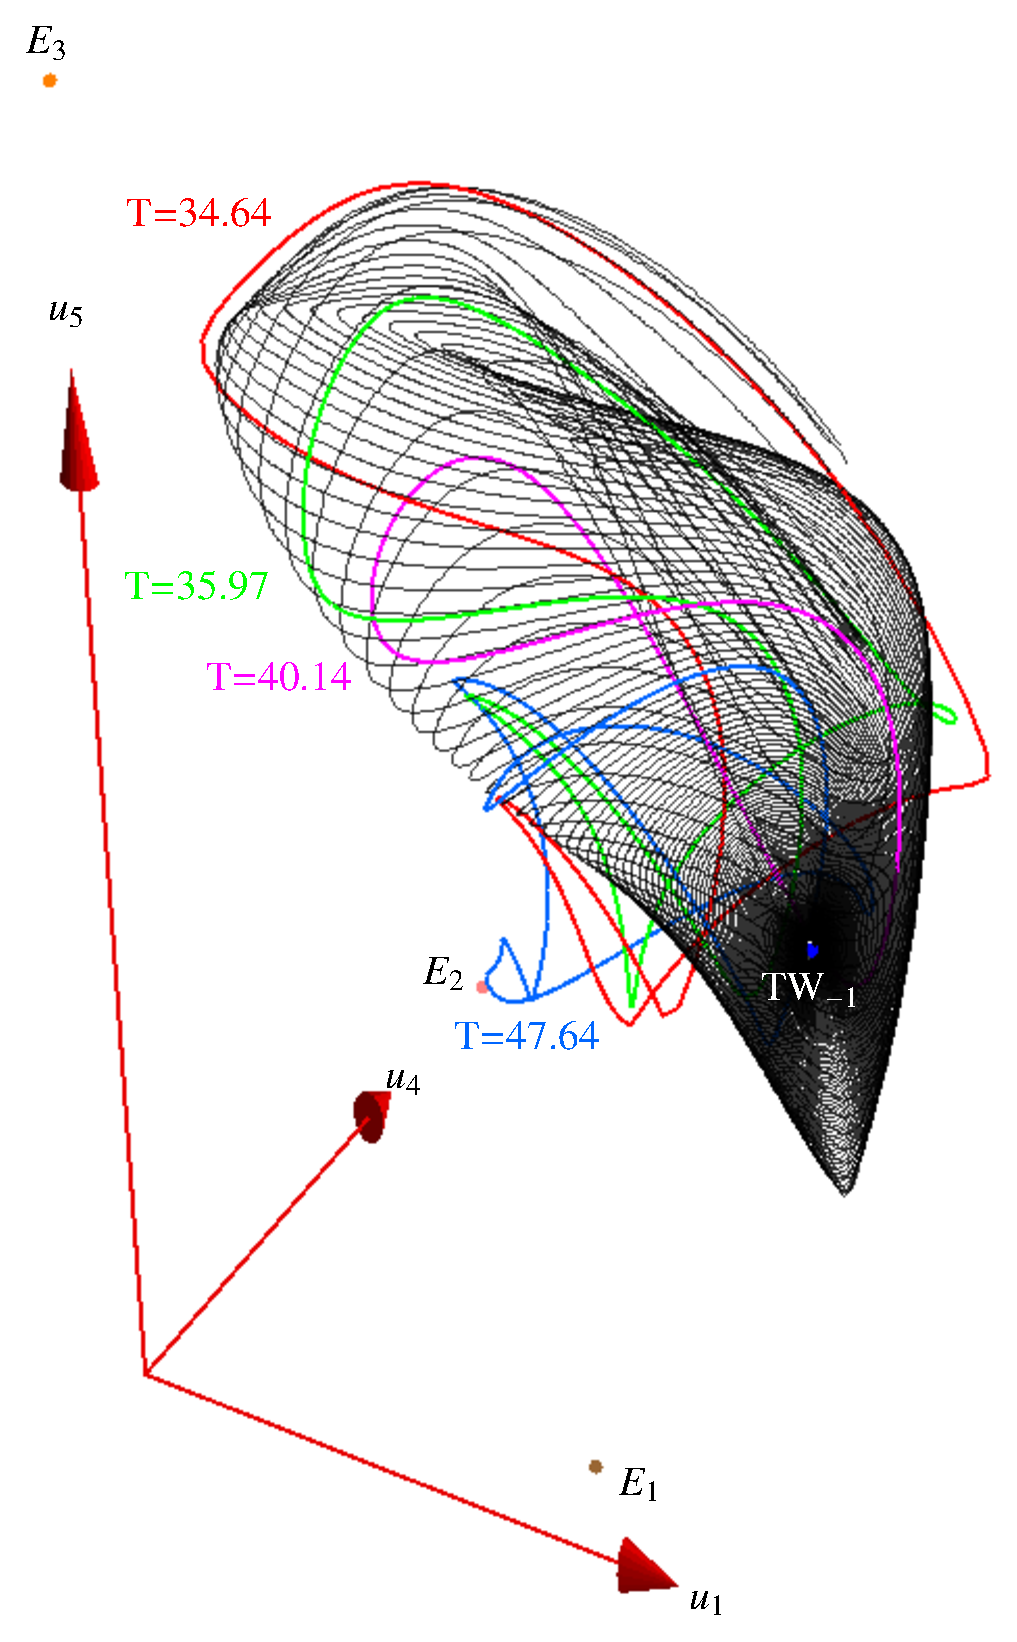
\includegraphics[width=0.9\textwidth, height=0.95\textheight,clip=true]{../../figs/ks22tw1umInv}
\column{0.5\textwidth}
	\only<1>{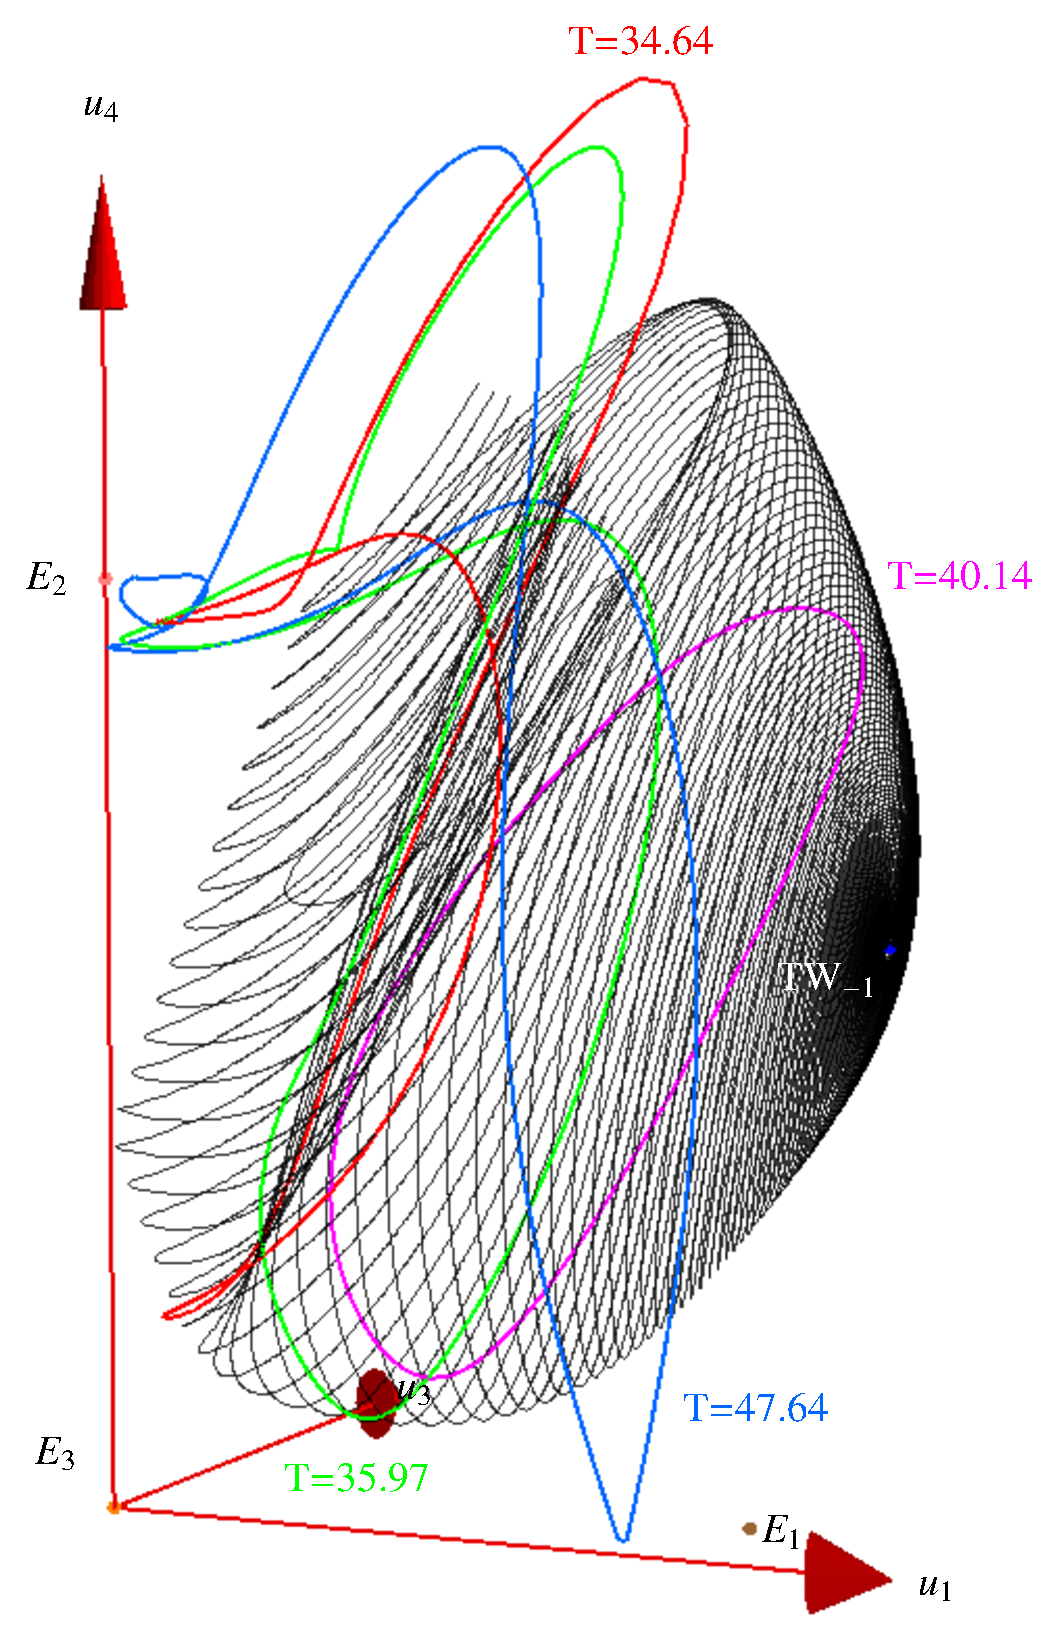
\includegraphics[width=\textwidth,height=0.95\textheight,clip=true]{../../figs/ks22tw1umInv2}}
	\only<2>{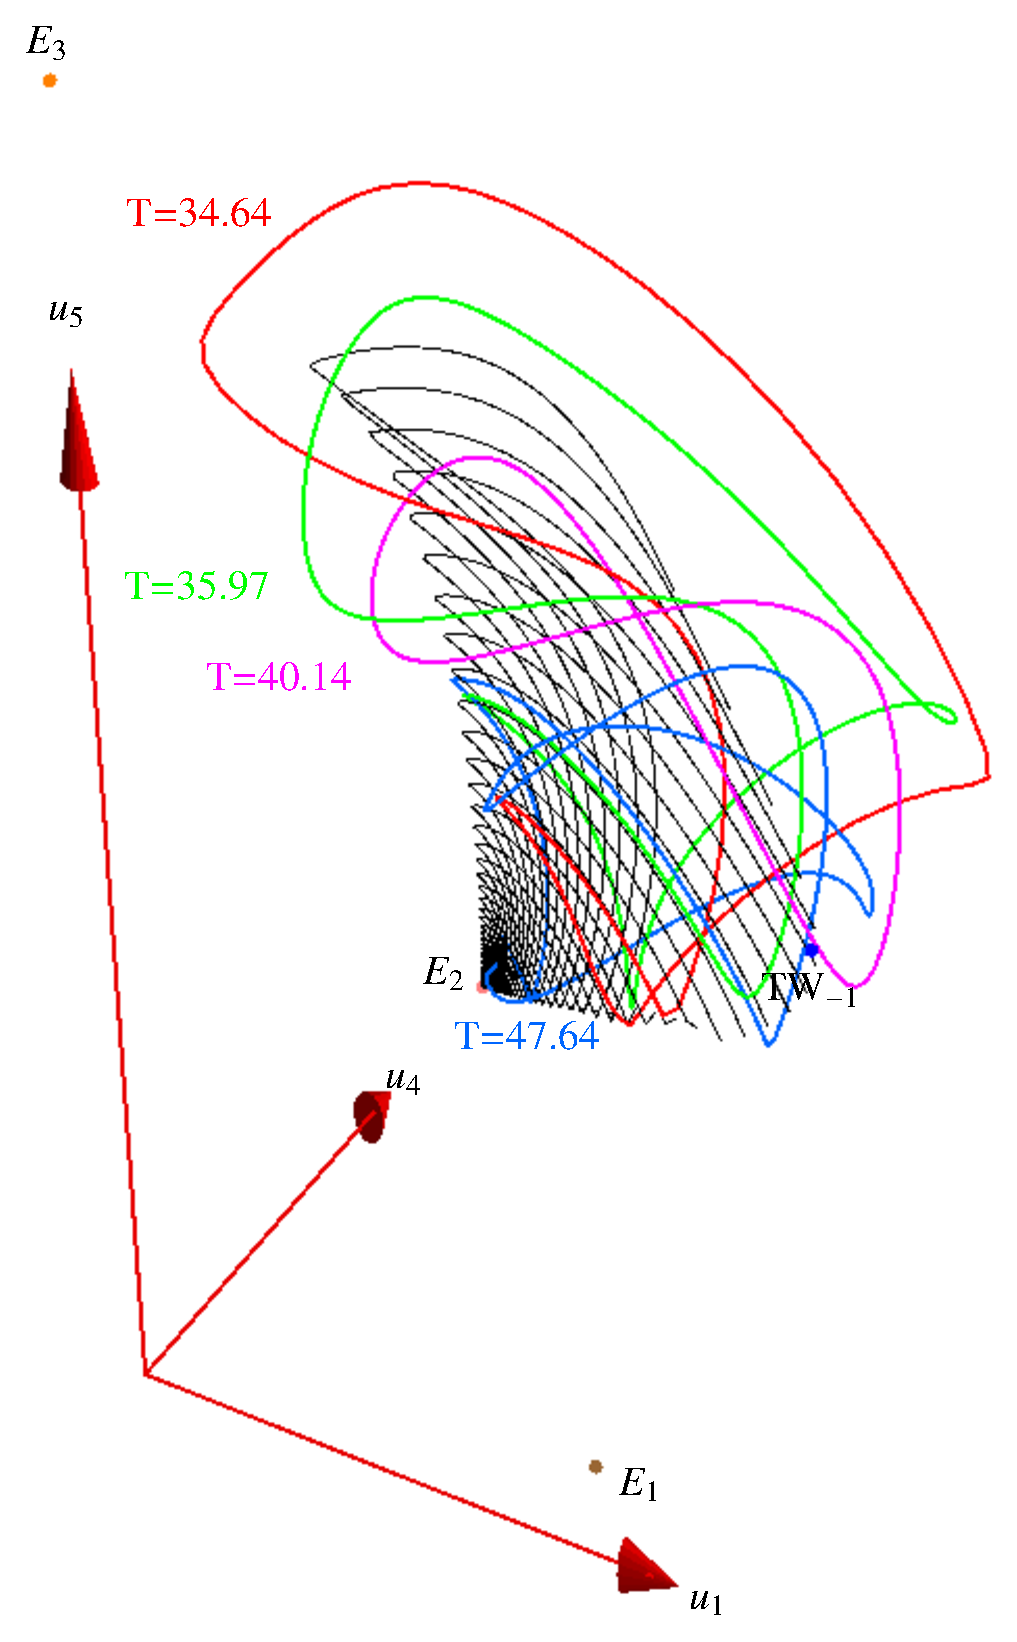
\includegraphics[width=\textwidth,height=0.95\textheight,clip=true]{../../figs/ks22-2wUMInv}} 
\end{columns}
\end{frame}

\section{Conclusions}
 
 \begin{frame}{Conclusions and future work}
 
\begin{block}{Conclusion}
  \begin{itemize}
   \item Symmetry reduction: efficient method allows exploration of high-dimensional flows with continuous symmetry.
   \item We develop an understanding of how the stretching and folding
  	of unstable manifolds in \KSe\ organizes the flow.
  \end{itemize}
\end{block}


\begin{block}{Future work}
\begin{itemize}
  \item Construct Poincar\'e sections and return maps from section to section.
  \item Find all (relative) periodic orbits up to a given period.
  \item Use the information quantitatively (periodic orbit theory).
\end{itemize}
\end{block}

\end{frame}

\begin{frame}{References}

\begin{itemize}
 \item {\sc Armbruster, D.}, {\sc Guckenheimer, J.}, and {\sc Holmes, P.},{\em
  SIAM J. Appl. Math.}, vol.~49, pp.~676--691, 1989.
 \item {\sc Brown, H.~S.} and {\sc Kevrekidis, I.~G.} in {\em Pattern Formation: Symmetry
  Methods and Applications}, vol.~5 of {\em Fields Inst. Commun.}, (Providence, RI), pp.~45--66,
  AMS, 1996.
 \item {\sc Fels, M.} and {\sc Olver, P.~J.}, {\em Acta Appl. Math.}, vol.~51, p.~161, 1998.
 \item {\sc Kevrekidis, I.~G.}, {\sc Nicolaenko, B.}, and {\sc Scovel, J.~C.}, {\em SIAM J. Appl. Math.}, vol.~50, no.~3, pp.~760--790, 1990.
 \item {\sc Cvitanovi{\'c}, P.}, {\sc Davidchack, R.~L.}, and {\sc Siminos, E.},
  {\tt arXiv:0709.2944}; {SIAM J. Applied Dynam. Systems}, to appear,
  2009.

\end{itemize}


 
\end{frame}


% \begin{frame}{}
% 
% % \begin{block}{}
% %  Application to Navier-Stokes is left as an exercise to the audience!
% % \end{block}
% 
% \end{frame}


\end{document}
